% Copyright (C) 2026: The University of Edinburgh, United Kingdom
%                 Authors: Craig Warren, Antonis Giannopoulos, John Hartley,
%                          and Nathan Mannall
%
% This file is part of gprMax.
%
% gprMax is free software: you can redistribute it and/or modify
% it under the terms of the GNU General Public License as published by
% the Free Software Foundation, either version 3 of the License, or
% (at your option) any later version.
%
% gprMax is distributed in the hope that it will be useful,
% but WITHOUT ANY WARRANTY; without even the implied warranty of
% MERCHANTABILITY or FITNESS FOR A PARTICULAR PURPOSE. See the
% GNU General Public License for more details.
%
% You should have received a copy of the GNU General Public License
% along with gprMax. If not, see <http://www.gnu.org/licenses/>.
%
% images_shared/yeecell2dTMz.tikz is the canonical editable source for this
% figure and images_shared/yeecell2dTMz.png. Convert the compiled PDF with
% `dvisvgm --pdf --no-fonts` before rasterising to preserve TeX glyphs.

\documentclass[tikz,border=4pt]{standalone}

\begin{document}
% Copyright (C) 2026: The University of Edinburgh, United Kingdom
%                 Authors: Craig Warren, Antonis Giannopoulos, John Hartley,
%                          and Nathan Mannall
%
% This file is part of gprMax.
%
% gprMax is free software: you can redistribute it and/or modify
% it under the terms of the GNU General Public License as published by
% the Free Software Foundation, either version 3 of the License, or
% (at your option) any later version.
%
% gprMax is distributed in the hope that it will be useful,
% but WITHOUT ANY WARRANTY; without even the implied warranty of
% MERCHANTABILITY or FITNESS FOR A PARTICULAR PURPOSE. See the
% GNU General Public License for more details.
%
% You should have received a copy of the GNU General Public License
% along with gprMax. If not, see <http://www.gnu.org/licenses/>.
%
% Input-ready TikZ source for the gprMax 2D TMz Yee-cell figure.
% The only required package is \usepackage{tikz}.

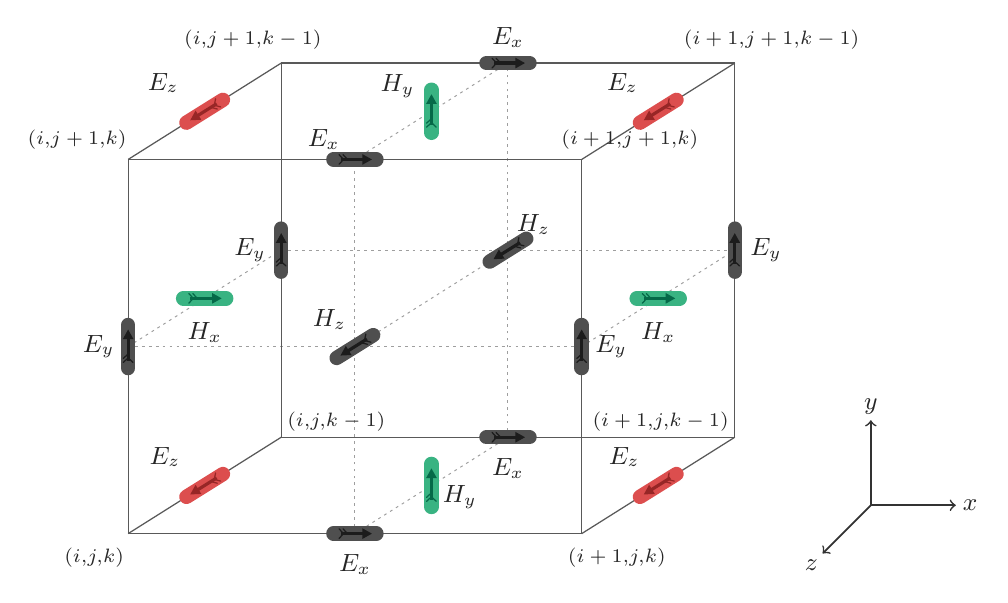
\begin{tikzpicture}[
    x=0.72cm,
    y=0.72cm,
    cell edge/.style={draw=black!65, line width=0.45pt},
    construction/.style={draw=black!38, line width=0.35pt, dash pattern=on 1pt off 1.5pt},
    field label/.style={font=\small\bfseries, text=black!85, inner sep=0pt},
    index label/.style={font=\scriptsize\bfseries\itshape, text=black!85, inner sep=0pt},
    axis label/.style={font=\small, text=black!85, inner sep=1pt}
]

\definecolor{yeeRed}{RGB}{220,78,78}
\definecolor{yeeRedDark}{RGB}{151,38,38}
\definecolor{yeeGreen}{RGB}{57,179,130}
\definecolor{yeeGreenDark}{RGB}{5,105,72}
\definecolor{yeeGrey}{RGB}{79,79,79}
\definecolor{yeeGreyDark}{RGB}{28,28,28}

% Compact, shadow-free field vector centred at #1 and rotated by #2 degrees.
\newcommand{\yeeField}[4]{%
  \begin{scope}[shift={#1}, rotate=#2]
    \draw[draw=#3, line width=5.2pt, line cap=round]
      (-0.38,0) -- (0.38,0);
    \fill[#4] (-0.25,-0.028) rectangle (0.15,0.028);
    \fill[#4] (0.30,0) -- (0.13,0.095) -- (0.13,-0.095) -- cycle;
    \draw[draw=#4, line width=0.45pt, line cap=round, line join=round]
      (-0.28,0.085) -- (-0.20,0) -- (-0.28,-0.085)
      (-0.21,0.085) -- (-0.13,0);
  \end{scope}%
}

% Front plane k and back plane k-1.
\coordinate (Fbl) at (0,0);
\coordinate (Fbr) at (8,0);
\coordinate (Ftl) at (0,6.6);
\coordinate (Ftr) at (8,6.6);
\coordinate (Bbl) at (2.7,1.7);
\coordinate (Bbr) at (10.7,1.7);
\coordinate (Btl) at (2.7,8.3);
\coordinate (Btr) at (10.7,8.3);

% Exact magnetic-face centres, defined from the face diagonals.
\path (Fbl) -- coordinate[midway] (HyBottom) (Bbr);
\path (Ftl) -- coordinate[midway] (HyTop) (Btr);
\path (Fbl) -- coordinate[midway] (HxLeft) (Btl);
\path (Fbr) -- coordinate[midway] (HxRight) (Btr);

% Cell-centre construction lines.
\begin{scope}[construction]
  \draw (4,0) -- (4,6.6) (0,3.3) -- (8,3.3);
  \draw (6.7,1.7) -- (6.7,8.3) (2.7,5) -- (10.7,5);
  \draw (0,3.3) -- (2.7,5);
  \draw (8,3.3) -- (10.7,5);
  \draw (4,0) -- (6.7,1.7);
  \draw (4,6.6) -- (6.7,8.3);
  \draw (4,3.3) -- (6.7,5);
\end{scope}

% Cell outline.
\draw[cell edge] (Fbl) -- (Fbr) -- (Ftr) -- (Ftl) -- cycle;
\draw[cell edge] (Bbl) -- (Bbr) -- (Btr) -- (Btl) -- cycle;
\draw[cell edge] (Fbl) -- (Bbl);
\draw[cell edge] (Fbr) -- (Bbr);
\draw[cell edge] (Ftl) -- (Btl);
\draw[cell edge] (Ftr) -- (Btr);

% Suppressed Ex components on x-directed edges.
\yeeField{(4,0)}{0}{yeeGrey}{yeeGreyDark}
\yeeField{(4,6.6)}{0}{yeeGrey}{yeeGreyDark}
\yeeField{(6.7,1.7)}{0}{yeeGrey}{yeeGreyDark}
\yeeField{(6.7,8.3)}{0}{yeeGrey}{yeeGreyDark}

% Suppressed Ey components on y-directed edges.
\yeeField{(0,3.3)}{90}{yeeGrey}{yeeGreyDark}
\yeeField{(8,3.3)}{90}{yeeGrey}{yeeGreyDark}
\yeeField{(2.7,5)}{90}{yeeGrey}{yeeGreyDark}
\yeeField{(10.7,5)}{90}{yeeGrey}{yeeGreyDark}

% Active Ez components on z-directed edges.
\yeeField{(1.35,0.85)}{-148}{yeeRed}{yeeRedDark}
\yeeField{(9.35,0.85)}{-148}{yeeRed}{yeeRedDark}
\yeeField{(1.35,7.45)}{-148}{yeeRed}{yeeRedDark}
\yeeField{(9.35,7.45)}{-148}{yeeRed}{yeeRedDark}

% Active Hx and Hy components, and suppressed Hz components.
\yeeField{(HxLeft)}{0}{yeeGreen}{yeeGreenDark}
\yeeField{(HxRight)}{0}{yeeGreen}{yeeGreenDark}
\yeeField{(HyBottom)}{90}{yeeGreen}{yeeGreenDark}
\yeeField{(HyTop)}{90}{yeeGreen}{yeeGreenDark}
\yeeField{(4,3.3)}{-148}{yeeGrey}{yeeGreyDark}
\yeeField{(6.7,5)}{-148}{yeeGrey}{yeeGreyDark}

% Field labels: Ex.
\node[field label] at (4,-0.55) {$E_x$};
\node[field label] at (3.45,6.95) {$E_x$};
\node[field label] at (6.7,1.15) {$E_x$};
\node[field label] at (6.7,8.75) {$E_x$};

% Field labels: Ey.
\node[field label] at (-0.52,3.3) {$E_y$};
\node[field label] at (8.52,3.3) {$E_y$};
\node[field label] at (2.15,5) {$E_y$};
\node[field label] at (11.25,5) {$E_y$};

% Field labels: Ez.
\node[field label] at (0.65,1.35) {$E_z$};
\node[field label] at (8.75,1.35) {$E_z$};
\node[field label] at (0.62,7.95) {$E_z$};
\node[field label] at (8.72,7.95) {$E_z$};

% Field labels: Hx, Hy, and Hz.
\node[field label] at (1.35,3.55) {$H_x$};
\node[field label] at (9.35,3.55) {$H_x$};
\node[field label] at (5.85,0.65) {$H_y$};
\node[field label] at (4.75,7.90) {$H_y$};
\node[field label] at (3.55,3.78) {$H_z$};
\node[field label] at (7.15,5.45) {$H_z$};

% Yee indices.
\node[index label] at (-0.60,-0.43) {$(i,\!j,\!k)$};
\node[index label] at (8.62,-0.43) {$(i+1,\!j,\!k)$};
\node[index label] at (-0.90,6.95) {$(i,\!j+1,\!k)$};
\node[index label] at (8.85,6.95) {$(i+1,\!j+1,\!k)$};
% Anchor the lower back-plane indices just inside their respective corners.
% This keeps the long labels clear of the diagonal Ez vectors.
\node[index label, anchor=south west, xshift=2pt, yshift=2pt]
  at (Bbl) {$(i,\!j,\!k-1)$};
\node[index label, anchor=south east, xshift=-2pt, yshift=2pt]
  at (Bbr) {$(i+1,\!j,\!k-1)$};
\node[index label] at (2.20,8.72) {$(i,\!j+1,\!k-1)$};
\node[index label] at (11.35,8.72) {$(i+1,\!j+1,\!k-1)$};

% Cartesian axes.
\draw[->, draw=black!80, line width=0.6pt] (13.1,0.5) -- (14.6,0.5);
\draw[->, draw=black!80, line width=0.6pt] (13.1,0.5) -- (13.1,2.0);
\draw[->, draw=black!80, line width=0.6pt] (13.1,0.5) -- (12.25,-0.35);
\node[axis label] at (14.85,0.5) {$x$};
\node[axis label] at (13.1,2.25) {$y$};
\node[axis label] at (12.05,-0.55) {$z$};

\end{tikzpicture}

\end{document}
